% SPDX-License-Identifier: Apache-2.0
%
% The brand lockup: the house mark plus a typeset wordmark. Used where the
% full logo is wanted; the site chrome uses brand-mark.* instead. Replace the
% wordmark text and/or the mark with your own. The wordmark is set in sans
% bold and vectorised to paths by dvisvgm (--no-fonts), so no font is needed
% at view time. Ink colour is injected by //bazel:tikz.bzl.
\def\pgfsysdriver{pgfsys-dvisvgm.def}
\documentclass[tikz,border=0pt]{standalone}
\begin{document}
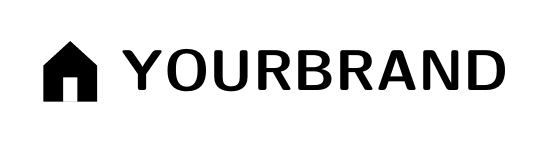
\begin{tikzpicture}[x=1mm, y=1mm]
  \draw[opacity=0,line width=0.01mm] (-0.4,-0.4) rectangle (52.0,10.4);
  % Mark: the same house glyph as brand-mark.tex, on the left.
  \fill[even odd rule]
    (1.6,1.0) -- (8.4,1.0) -- (8.4,5.6) -- (5.0,8.7) -- (1.6,5.6) -- cycle
    (4.1,1.0) -- (5.9,1.0) -- (5.9,4.1) -- (4.1,4.1) -- cycle;
  % Wordmark: replace "YOURBRAND" with your name.
  \node[anchor=west, inner sep=0pt] at (11.5,4.9)
    {\fontsize{22}{22}\selectfont\sffamily\bfseries YOURBRAND};
\end{tikzpicture}
\end{document}
